%!TEX root = ../DevaramaniS-[RnD-MT]Report.tex

\chapter{Methodology} 
This chapter describes the applied robot platform used to test the extended solver. To begin with, the robot has to be modeled as a kinematic tree structure. Therefore, the following sections briefly discuss the applied robot specifications and further describes the representation of this robot as a kinematic tree structure. 




\section{Robot Specifications}
The applied robot platform is MPO-700 (figure \ref{fig:MPO-700})~\cite{MPO700}. MPO-700 is an omni-directional base employed in high-end service robots~\cite{Neobotix-homepage}. The base features four \textit{Neobotix omnidirectional modules} that enables smooth motion in X-Y directions. When compared to other robot bases with omnidirectional drive kinematics, the MPO-700 has great maneuverability, steadiness, high stability and compact~\cite{Neobotix-homepage}. Hence, it is used in wide range of applications. One of the popular platform built based of MPO-700 is \textit{Care-O-bot} 3 developed by Fraunhofer IPA\footnote{Fraunhofer IPA - \url{http://www.ipa.fraunhofer.de}}. 


\paragraph{}The MPO-700 base has four Castor wheels and four drive wheels. The drive wheels are at an offset from castor wheels. In the default configuration, the drive wheels are oriented inwards by $45^0$ (as seen in figure \ref{fig:MPO-700}). A controlled motion can only be acheieved if all the drives coordinated properly. The robot base is also equipped with two SICK sensors (laser scanners), whose data is used for obstacle avoidance. There are two emergency stop buttons placed on either side of the base. In case of danger, the robot motion can be stopped immediately by pressing these emergency buttons. On the base, there is a LC-Display, which displays the detailed information on current state of the robot. A key witch is present slightly above laser scanner. This is used to start or stop the robot~\cite{MPO700}.

\begin{figure}[h!]
	\centering	
	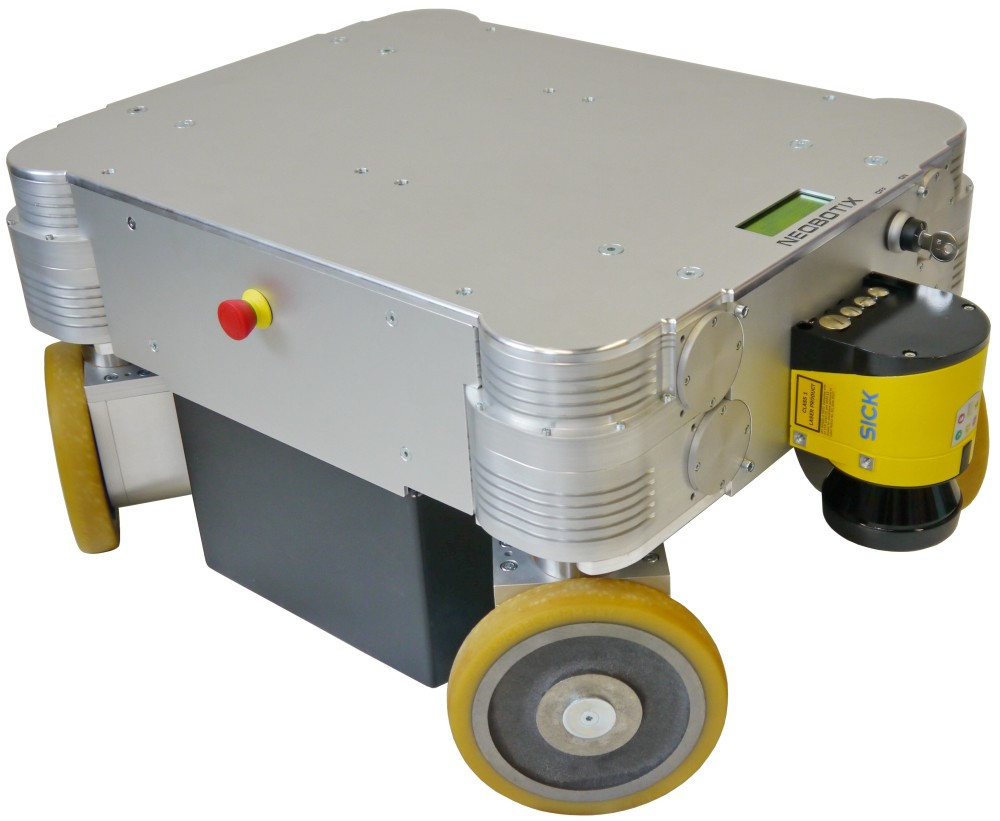
\includegraphics[scale=0.5]{images/mp0700}
	\caption{MPO-700 Neobotix (source: \cite{MPO700-Datasheet})}
	\label{fig:MPO-700}
\end{figure}

%For modeling MPO-700 as tree, the base is defined as root of the kinematic tree. Further, individual segments, defined as KDL::Segment are connected to the \textit{root}. Using the technical dimensions from the MPO-700 operating manual~\cite{MPO700}, each of the segments are defined.



%\section{Software Specifications}
%Currently the Vereshchagin solver for kinematic chains is implemented in \hyperref[kdl]{KDL} library~\cite{KDLopensource} using C++ programming language. In our implementation, after modeling the MPO-700 robot base as kinematic tree structure, the current code base is extended according to the proposed algorithm in the chapter \ref{chap:extension}.

\section{Kinematic Tree Representation}

A kinematic tree comprises of interconnected segments (links). A typical kinematic tree description is provided by \hyperref[kdl]{KDL} library. Representation of a single segment (KDL::Segment) is given in figure \ref{fig:segment}~\cite{kinematictreeKDL}.

\begin{figure}[h!]
	\begin{center}
		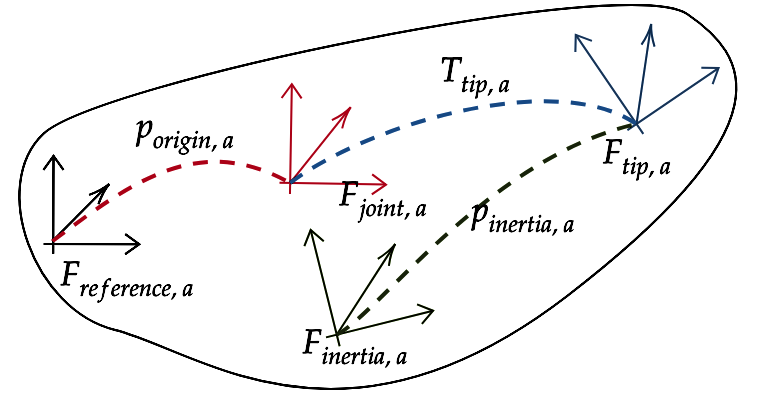
\includegraphics[scale=0.25]{images/segment}
	\end{center}
	\caption{KDL Segment (source: \cite{kinematictreeKDL})}
	\label{fig:segment}
\end{figure} 

\paragraph{}A KDL segment (figure:\ref{fig:segment}) is composed of four frames,
\begin{enumerate}
	\item $F_{reference}$: A \textit{reference} frame (black colored frame) with respect to which other frames are expressed.
	\item $F_{joint}$: A one DOF \textit{joint} frame (red) expressed about joint axis. The orientation of the frame is same as $\{F_{reference}\}$ and translation is given by $\{p_{origin, a}\}$. The frame is defined in KDL::Joint class.
	\item $F_{inertia}$: A \textit{Cartesian space inertia matrix} (green) expressed with respect to \textit{tip frame} and $p_{inertia, a}$ is the translation vector. The frame is defined in KDL::RigidBodyInertia class.  
	\item $F_{tip}$: Frame attached at the tip of a segment. As seen in the figure \ref{fig:segment}, $\{F_{tip, a}\}$ is defined with respect to joint frame (blue) and transformation is given by $\{T_{tip, a}\}$ (by default: $\{T_{tip, a}\}$ is identity transformation). 
\end{enumerate}

\paragraph{}A Kinematic tree is simply a composition of these KDL segments. An example is shown in the below figure (\ref{fig:kinematic-tree}) which describes a \textit{Kinematic tree} with two branches~\cite{kinematictreeKDL}. Here, \textit{Segment a} is the \textit{root} of the tree and \textit{Segment b} and \textit{Segment c} are \textit{child branches}. According to the convention, the joint frame of the succeeding segment is attached to tip frame of the preceding segment. Therefore, the tip frames acts as the reference frame for the succeeding segments ($F_{tip, a} = F_{reference, b} = F_{reference, c}$). Similarly, the representation can be extended for multiple chains and interconnected segments. Referring to this representation, a tree structure for the MPO-700 base is created in next section.

\begin{figure}[h]
	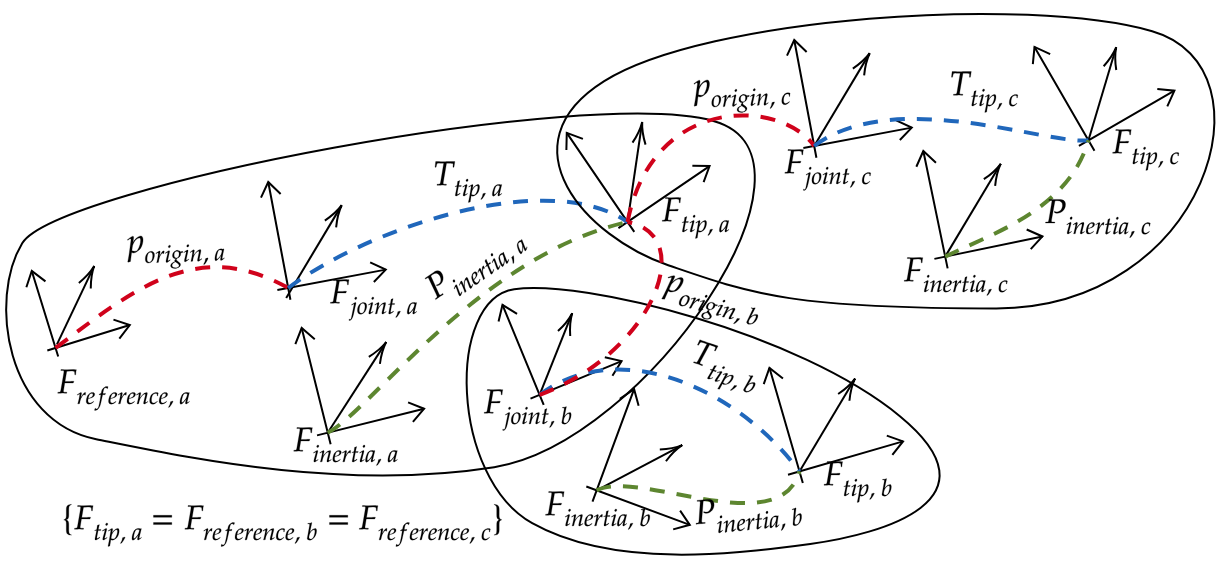
\includegraphics[scale=0.36]{images/kinematic-tree}
	\caption{Kinematic tree representation in KDL (source: \cite{kinematictreeKDL})}
	\label{fig:kinematic-tree}
\end{figure}

\newpage
\subsection{MPO-700 base as kinematic tree}
The MPO-700 robot base is modeled as kinematic tree by defining the robot chassis as \textit{root} of the tree. As seen in the figure \ref{fig:tree-MPO}, the \textit{root frame} is defined at the center, on the surface of chassis. Using the technical dimensions obtained from the operating manual and URDF model of base, further tree elements are designed~\cite{MPO700}. 

A sub-chain is defined from root to the drive wheel's point of contact on the ground. Each of these sub-chains comprises of three segments. However, only the \textit{tip frame} of the segments are shown in the figure. One of the sub-chains is explained below.

\begin{figure}[h!]
	\begin{center}
		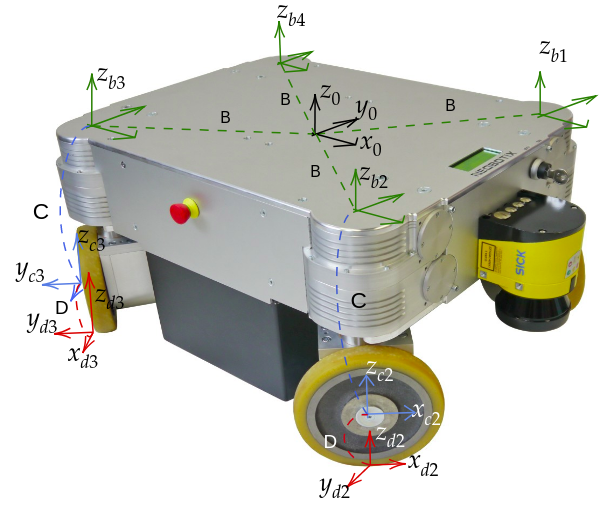
\includegraphics[scale=0.45]{images/MPO-700-tree}
	\end{center}	
	\caption{Representation of tree structure on MPO-700 [source: \cite{MPO700-Datasheet}](Note: The links with same name represents identical transformation)}
	\label{fig:tree-MPO}
\end{figure}

\begin{itemize}
	\item B: represents link from root frame to the frame (green) at the corner of the chassis. Physically this link denotes translation from tip of root segment to tip of segment B2. Here, the $z_{b2}$ axis coincides with the castor wheel's axis.
	\item C: denotes a link from corner of the chassis ($z_{b2}$) to the center of the drive wheel ($z_{c2}$). Please note that the drive wheel is at an offset from castor and is oriented by $45^0$. Hence, C2 represents transformation between these two frames.
	\item D: defines the link from center of drive wheel to its point of contact on the ground. Physically, D represents the wheel radius. 
\end{itemize}



\paragraph{}The KDL::Tree class adds all the sub-chains to the root segment. A 2D view of this tree structure is shown in the figure \ref{fig:planar-tree}. As previously mentioned, the outward and inward recursions are achieved similar to \textit{breadth-first search} and \textit{reverse breadth-first search} respectively. The tree elements must be ordered in such a way that, the recursion imitates these search patterns. When the tree structure is created, the KDL::SegmentMap function arranges the tree elements lexicographically. Hence, the segment names follow lexicographical order (as seen in figure \ref{fig:planar-tree}).  

\begin{figure}[h!]
	\begin{center}
		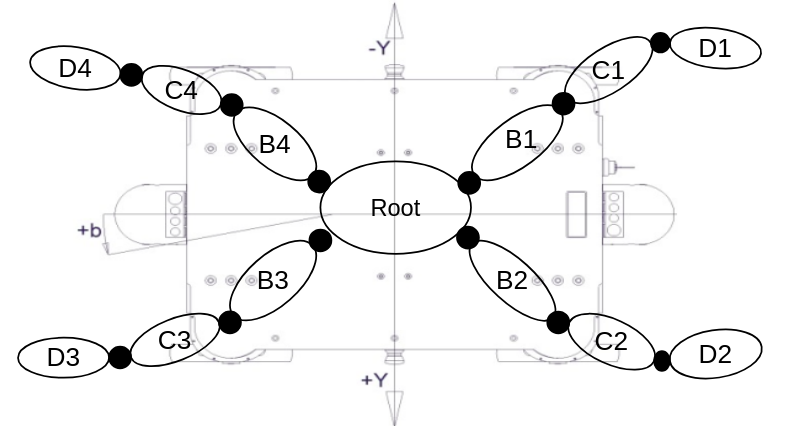
\includegraphics[scale=0.45]{images/kinematic-tree-MPO-700}
	\end{center}	
	\caption{Kinematic tree structure of MPO-700 robot base (source: \cite{MPO700})}
	\label{fig:planar-tree}
\end{figure}

\newpage
\section{Implementation details}
Currently the Vereshchagin solver for kinematic chains is implemented in \hyperref[kdl]{KDL} library~\cite{KDLopensource} using C++ programming language. The available code base for the current solver is developed and maintained by the Ruben Smits, Herman Bruyninckx, Azamat Shakhimardanov~\cite{KDLopensource}. In the chapter~\ref{chap:extension}, the extended algorithm for kinematic tree was proposed.  Further interest lies in implementing this proposed algorithm on MPO-700 robot base. As described above, the robot base is modeled as tree structure in KDL library. Further, the existing code base is extended to implement the proposed algorithm. 

%\begin{figure}[h!]
%	\centering
%	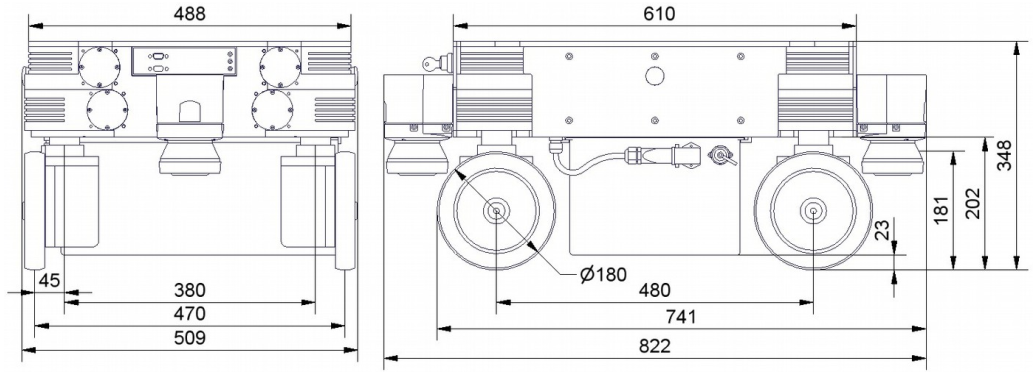
\includegraphics[scale=0.4]{images/technicaldata}
%	\caption{MPO-700 dimensions (source:~\cite{MPO700-Datasheet})}
%	\label{fig:Technicaldata}
%\end{figure}
%
%\begin{figure}[h!]
%	\centering
%	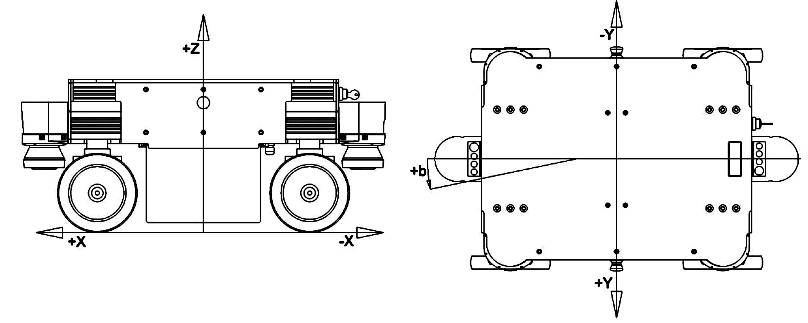
\includegraphics[scale=0.4]{images/coordinate}
%	\caption{MPO-700 Coordinate system convention (source:~\cite{MPO700})}
%	\label{fig:coordinate}
%\end{figure}
%To define a physical link as KDL::Segment, The required information to describe a physical link as a KDL::Segment are, 




